%structure taken from the fischsheet https://bitbucket.org/toman/fischsheet

%template by http://stdout.org/~winston/latex/

\documentclass[10pt,landscape,a4paper]{article}
\usepackage{multicol}
\usepackage{calc}
\usepackage{ifthen}
\usepackage[landscape]{geometry}
\usepackage{amsmath,amsthm,amsfonts,amssymb}
\usepackage{color,graphicx,overpic}
\usepackage{hyperref}
\usepackage{txfonts}
\usepackage[latin1]{inputenc}
\usepackage[T1]{fontenc}
\usepackage[ngerman]{babel}
\usepackage{listings}
\usepackage{pdfpages}
\lstset{tabsize = 3}


\pdfinfo{
  /Title (Cheatsheet #define true false)
  /Creator (TeX)
  /Author (Lukas, Quirin, Sebastian)
  /Subject (Cheatsheet for NWERC 2014)
}

% This sets page margins to .5 inch if using letter paper, and to 1cm
% if using A4 paper. (This probably isn't strictly necessary.)
% If using another size paper, use default 1cm margins.
\geometry{top=.45in,left=.5in,right=.5in,bottom=.5in}

% Turn off header and footer
\pagestyle{empty}

% Redefine section commands to use less space
\makeatletter
\renewcommand{\section}{\@startsection{section}{1}{0mm}%
                                {-1ex plus -.5ex minus -.2ex}%
                                {0.5ex plus .2ex}%x
                                {\normalfont\large\bfseries}}
\renewcommand{\subsection}{\@startsection{subsection}{2}{0mm}%
                                {-1explus -.5ex minus -.2ex}%
                                {0.5ex plus .2ex}%
                                {\normalfont\normalsize\bfseries}}
\renewcommand{\subsubsection}{\@startsection{subsubsection}{3}{0mm}%
                                {-1ex plus -.5ex minus -.2ex}%
                                {1ex plus .2ex}%
                                {\normalfont\small\bfseries}}
\makeatother

% Define BibTeX command
\def\BibTeX{{\rm B\kern-.05em{\sc i\kern-.025em b}\kern-.08em
    T\kern-.1667em\lower.7ex\hbox{E}\kern-.125emX}}

% Don't print section numbers
\setcounter{secnumdepth}{0}


\setlength{\parindent}{0pt}
\setlength{\parskip}{0pt plus 0.5ex}

%My Environments
\newtheorem{example}[section]{Example}
% -----------------------------------------------------------------------

\usepackage{fancyhdr}
\pagestyle{fancy}
\setlength{\headheight}{17pt} 
\lhead{Technische Universit\"at M\"unchen}
\rhead{\thepage}
\fancyfoot{}

\begin{document}
\raggedright
\footnotesize
\begin{multicols}{2}


% multicol parameters
% These lengths are set only within the two main columns
%\setlength{\columnseprule}{0.25pt}
\setlength{\premulticols}{1pt}
\setlength{\postmulticols}{1pt}
\setlength{\multicolsep}{1pt}
\setlength{\columnsep}{2pt}

\begin{center}
     \Large{
     	Team Reference Document\\
     	\underline{Team \#define true false, TU M\"unchen}\\
     	NWERC 2014} \\
\end{center}

\tableofcontents


\section{Computations}
\subsection{Greates Common Divisor}

\begin{lstlisting}
long gcd(long a, long b)
{
if (b == 0)
return a;
else return gcd(b, a % b);
}
\end{lstlisting}

\subsection{Binomial Coefficients}

\begin{lstlisting}
long binomial(long n, long k)
{
if (k > n - k)
return binomial(n, n - k);

long result = 1;
if (k > n)
return 0;

for (long next = 1; next <= k; ++next)
{
long cancelled = gcd(result, next);
result = (result / cancelled)*(n - next + 1);
result = result/(next/cancelled);
}

return result;
}
\end{lstlisting}

\section{Flow}
\subsection{MaxFlow Push-Relabel}

\begin{lstlisting}
#include <cmath>
#include <vector>
#include <iostream>
#include <queue>
using namespace std;
typedef long long LL;

struct Edge {
  int from, to, cap, flow, index;
  Edge(int from, int to, int cap, int flow, int index) :
    from(from), to(to), cap(cap), flow(flow), index(index) {}
};

struct PushRelabel {
  int N;
  vector<vector<Edge> > G;
  vector<LL> excess;
  vector<int> dist, active, count;
  queue<int> Q;

  PushRelabel(int N) : N(N), G(N), excess(N), dist(N), active(N), count(2*N) {}

  void AddEdge(int from, int to, int cap) {
    G[from].push_back(Edge(from, to, cap, 0, G[to].size()));
    if (from == to) G[from].back().index++;
    G[to].push_back(Edge(to, from, 0, 0, G[from].size() - 1));
  }

  void Enqueue(int v) { 
    if (!active[v] && excess[v] > 0) { active[v] = true; Q.push(v); } 
  }

  void Push(Edge &e) {
    int amt = int(min(excess[e.from], LL(e.cap - e.flow)));
    if (dist[e.from] <= dist[e.to] || amt == 0) return;
    e.flow += amt;
    G[e.to][e.index].flow -= amt;
    excess[e.to] += amt;    
    excess[e.from] -= amt;
    Enqueue(e.to);
  }
  
  void Gap(int k) {
    for (int v = 0; v < N; v++) {
      if (dist[v] < k) continue;
      count[dist[v]]--;
      dist[v] = max(dist[v], N+1);
      count[dist[v]]++;
      Enqueue(v);
    }
  }

  void Relabel(int v) {
    count[dist[v]]--;
    dist[v] = 2*N;
    for (int i = 0; i < G[v].size(); i++) 
      if (G[v][i].cap - G[v][i].flow > 0)
	dist[v] = min(dist[v], dist[G[v][i].to] + 1);
    count[dist[v]]++;
    Enqueue(v);
  }

  void Discharge(int v) {
    for (int i = 0; excess[v] > 0 && i < G[v].size(); i++) Push(G[v][i]);
    if (excess[v] > 0) {
      if (count[dist[v]] == 1) 
	Gap(dist[v]); 
      else
	Relabel(v);
    }
  }

  LL GetMaxFlow(int s, int t) {
    count[0] = N-1;
    count[N] = 1;
    dist[s] = N;
    active[s] = active[t] = true;
    for (int i = 0; i < G[s].size(); i++) {
      excess[s] += G[s][i].cap;
      Push(G[s][i]);
    }
    
    while (!Q.empty()) {
      int v = Q.front();
      Q.pop();
      active[v] = false;
      Discharge(v);
    }
    
    LL totflow = 0;
    for (int i = 0; i < G[s].size(); i++) totflow += G[s][i].flow;
    return totflow;
  }
};

\end{lstlisting}

% You can even have references
%\rule{0.3\linewidth}{0.25pt}
\scriptsize
%\bibliographystyle{abstract}
%\bibliography{refFile}
\end{multicols}
\newpage
\addcontentsline{toc}{section}{Theoretical CS Cheat Sheet}
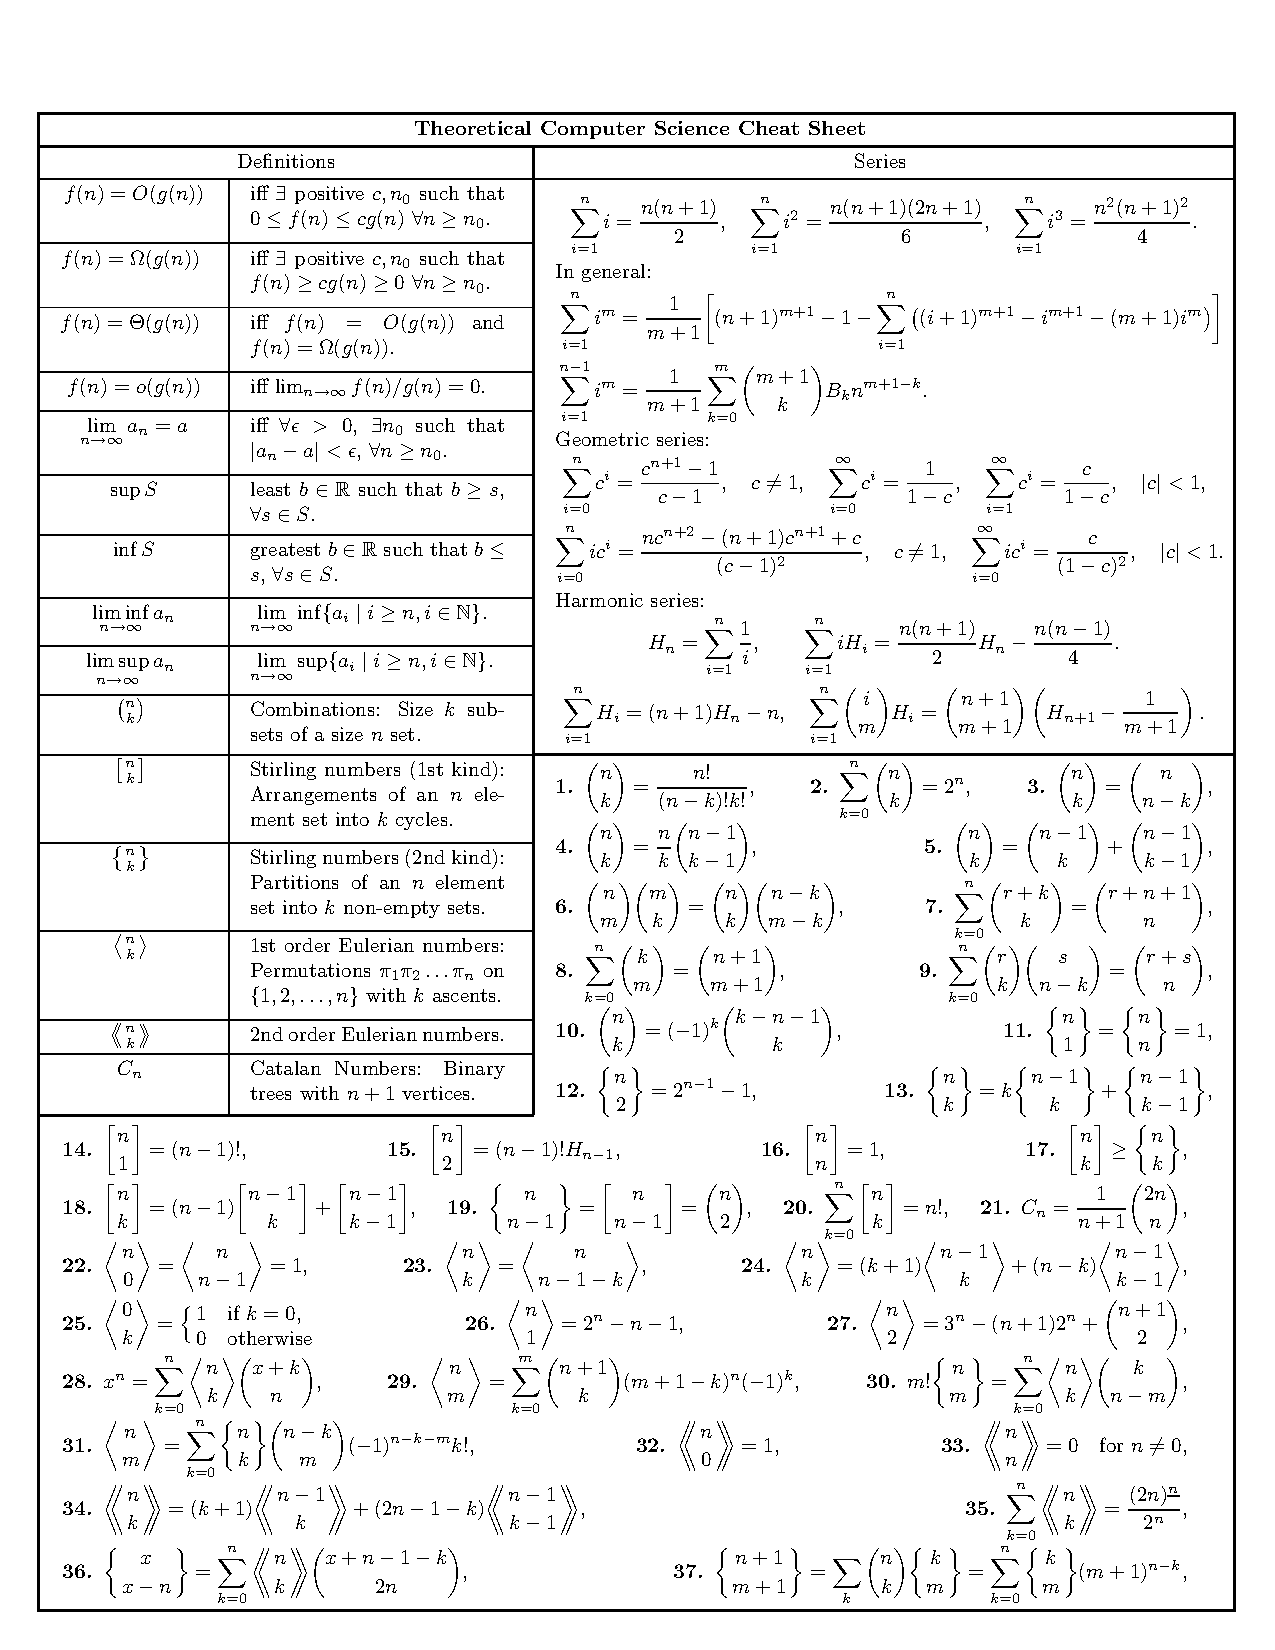
\includepdf[landscape=true,pages={1-5},pagecommand={\thispagestyle{fancy}}]{cheat}

\end{document}